\documentclass[conference]{IEEEtran}
\usepackage{times}
\usepackage{graphicx}
\usepackage{tikz}
\usepackage{mathtools, amsfonts, breqn, subcaption}
\usepackage{tabu}
\DeclareMathOperator*{\argmin}{arg\,min}

% numbers option provides compact numerical references in the text. 
\usepackage[numbers]{natbib}
\usepackage{multicol}
\usepackage[bookmarks=true]{hyperref}

\pdfinfo{
   /Author (Varun Murali)
   /Title  (Evaluation of Safe Control Policies for Mobile Robots in Dynamic Environments)
   /CreationDate (D:20101201120000)
   /Subject (Safe Robotics)
   /Keywords (Safety Control)
}

\begin{document}

% paper title
\title{Evaluation of Safe Control Policies for \\Mobile Robots in Dynamic Environments }

% You will get a Paper-ID when submitting a pdf file to the conference system
\author{Varun~Murali, Niharika~Arora, Ian~Buckley}

%\author{\authorblockN{Michael Shell}
%\authorblockA{School of Electrical and\\Computer Engineering\\
%Georgia Institute of Technology\\
%Atlanta, Georgia 30332--0250\\
%Email: mshell@ece.gatech.edu}
%\and
%\authorblockN{Homer Simpson}
%\authorblockA{Twentieth Century Fox\\
%Springfield, USA\\
%Email: homer@thesimpsons.com}
%\and
%\authorblockN{James Kirk\\ and Montgomery Scott}
%\authorblockA{Starfleet Academy\\
%San Francisco, California 96678-2391\\
%Telephone: (800) 555--1212\\
%Fax: (888) 555--1212}}


% avoiding spaces at the end of the author lines is not a problem with
% conference papers because we don't use \thanks or \IEEEmembership


% for over three affiliations, or if they all won't fit within the width
% of the page, use this alternative format:
% 
%\author{\authorblockN{Michael Shell\authorrefmark{1},
%Homer Simpson\authorrefmark{2},
%James Kirk\authorrefmark{3}, 
%Montgomery Scott\authorrefmark{3} and
%Eldon Tyrell\authorrefmark{4}}
%\authorblockA{\authorrefmark{1}School of Electrical and Computer Engineering\\
%Georgia Institute of Technology,
%Atlanta, Georgia 30332--0250\\ Email: mshell@ece.gatech.edu}
%\authorblockA{\authorrefmark{2}Twentieth Century Fox, Springfield, USA\\
%Email: homer@thesimpsons.com}
%\authorblockA{\authorrefmark{3}Starfleet Academy, San Francisco, California 96678-2391\\
%Telephone: (800) 555--1212, Fax: (888) 555--1212}
%\authorblockA{\authorrefmark{4}Tyrell Inc., 123 Replicant Street, Los Angeles, California 90210--4321}}


\maketitle

\begin{abstract}
With the growth of domestic robot industry, it is important to understand the navigation of mobile robots in dynamic environments. Use of mobile robots in the home can greatly improve the quality of life and is a growing field of research. With an increased interaction between humans and robots, and an increasingly shared workspace, it is important to study the safety of the robotic system and the extent of guarantees that can be made to minimize risk of injury. We present a nonlinear control approach to the navigation problem that achieves the objective of reaching pre-defined locations with provable guarantees of safety. Verification of the controller is performed first in MATLAB simulation, which shows that the controller is capable of driving the system to a pre-defined location while maintaining all required safety rules defined in it's environment. The system is implemented on a Segway RMP 200 based robot, demonstrating that the nonlinear navigation controller successfully traverses the gap between theory and practice. 
\end{abstract}

\IEEEpeerreviewmaketitle

\section{Introduction}
Safety is an important concern for mobile robots working in collaborative environments. Typical robotic systems separately deal with safety and task completion in a hierarchical fashion--a high level controller decides which control law to use based on the situation. Navigation is of fundamental concern for mobile robots. The ability to successfully avoid obstacles, both static and dynamic, while moving towards a goal location largely determines the utility of a mobile robotic platform. It is critical that robots avoid obstacles for their own safety as well as the safety of the people around them. We use the navigation problem to motivate the direct addition of safety into the controller for the robot.

After formulating the navigation control strategy, MATLAB simulation is used to verify that the navigation control strategy correctly drives the state of the robot to a target. After demonstrating that the robot successfully navigates to a target location, a trajectory is generated for a map using a probabilistic roadmap, and the navigation control strategy is used to drive the robot along the trajectory. After thoroughly substantiating the efficacy of the navigation control strategy in simulation, the controller is implemented in the ROS framework and evaluated on a Segway RMP 200 based mobile robot, verifying the navigation control strategy in a real world scenario.

\section{Approach}
Control Lyapunov functions and control barrier functions are formulated to individually accomplish the objectives of navigation and obstacle avoidance. The control Lyapunov and barrier functions are soft and hard constrained in a Quadratic Programming based controller to achieve safe navigation. Figure~\ref{fig:obs} shows the egocentric coordinate system of the robot and describes the variables used in the polar form of the unicycle dynamics modelling the robot, given by: 
\begin{equation}
\left(
\begin{matrix}
\dot{r}\\
\dot{\theta}\\
\end{matrix}
\right)
=
\left(
\begin{matrix}
- v \text{ cos}(\delta)\\
\frac{v}{r} \text{ sin}(\delta)\\
\end{matrix}
\right).
\end{equation}
\begin{equation}
\dot{\delta}=\frac{v}{r} \text{ sin}(\delta)+\omega
\end{equation}
\begin{figure}[t]
\begin{center}
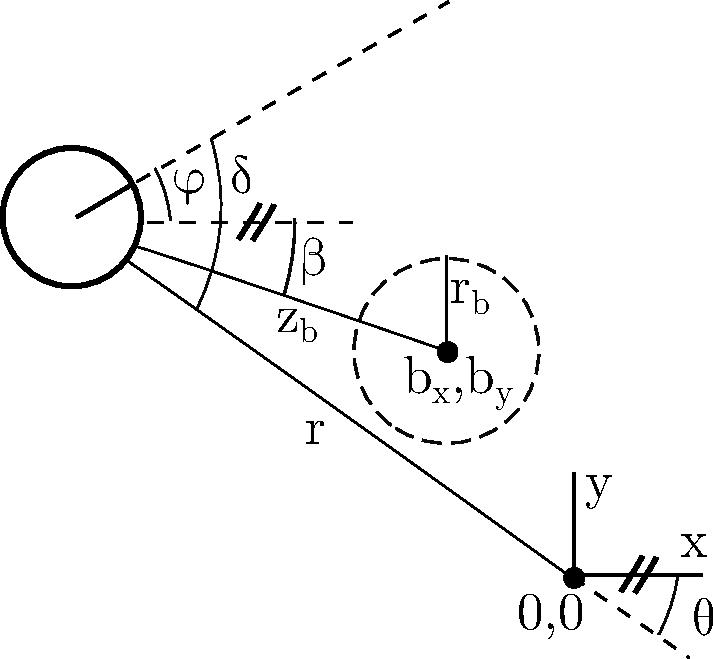
\includegraphics[scale=0.35]{obs.pdf} 
\caption{The egocentric co-ordinate system of the robot is shown above. $r$ is the radial distance of the robot from the origin, $\phi$ is the heading of the robot in the target frame, $\theta$ is the orientation of the target frame in the robot frame, and $\delta$ is  the egocentric heading. $\beta$ is the angle between the global $x$-axis and the vector joining the center of the robot to the obstacle. \label{fig:obs}} 
\end{center}
\end{figure}

\subsection{Control Lyapunov Functions}
To design the control law, the standard quadratic Lyapunov function candidate is first considered:
\begin{align}
V&=\frac{1}{2}(r^2+\theta^2)\\
\dot{V}&=r \dot{r}+\theta \dot{\theta}\\
&=-r v \text{ cos}(\delta) + \theta v \text{ sin}(\delta)
\end{align}
Fixing $\delta$ to enforce a virtual steering control as in \cite{park2011}, 
\begin{equation} 
\delta = \text{arctan}(-k_1\theta). \end{equation}
The derivative of the Lyapunov function becomes:
\begin{equation}
\dot{V}=-r v \text{ cos}(\text{arctan}(-k_1\theta)) + \theta v \text{ sin}(\text{arctan}(-k_1\theta)).
\end{equation} 

%Furthermore, by the definition of the steering control, $\delta\to 0$ as $\theta \to 0$, so the virtual steering control not only drives the robot to the final position, but aligns the heading of the robot with the positive $x$-axis of the global coordinate frame by the time it arrives at the final position.
Because $\theta\in (-\pi,\pi]$, $v>0$, and $r\geq 0$ , $\dot{V}<0$ $\forall \theta$, $r\neq0$; thus, the steering control asymptotically drives $r,\theta\to 0$. By choosing $v=k_3 r$ in some neighborhood of $r=0$ for positive constant $k_3,$ the singularity at $r=0$ is removed and the system is globally asymptotically stable.  Furthermore, the virtual steering control simultaneously drives the robot to the final position while aligning its heading with the positive global $x$-axis. 

To drive the state to zero through the steering control, the heading must be driven such that $\delta = \text{arctan}(-k_1\theta).$ An objective $z_1$ is defined: 
\begin{equation}
z_1 \equiv \delta - \text{arctan}(-k_1\theta).
\label{z1}
\end{equation} The derivative is calculated to yield:
\begin{equation}
\dot{z_1}=\left( 1+\frac{k_1}{1+(k_1\theta)^2}\right) \frac{v}{r}\text{ sin}(z_1+\text{ arctan}(-k_1\theta))+\omega.
\end{equation}
Feedback linearization can be used to achieve this objective by choosing the angular velocity 
\begin{equation}
\begin{split}
\omega = -\frac{v}{r}\left[ k_2 z_1+\left( 1 + \frac{k_1}{1+(k_1\theta)^2} \right)\right.\\
\left. \vphantom{\frac{v}{r}} \text{sin}(z_1+\text{ arctan}(-k_1\theta))\right],
\end{split}
\end{equation}
the objective dynamics are globally exponentially stable with the following form: \begin{equation} \dot{z_1}=-k_2\frac{v}{r}z_1,\end{equation} where $k_1$ and $k_2$ can be chosen to increase or decrease how aggressive the steering control is. This is modelled along with other constraints by defining: 
\begin{equation} V_2 = \frac{1}{2}  z^2. \end{equation}

A second steering controller is designed to drive the state away from the origin and is defined by the following objective: \begin{equation}z_2=\delta-\text{ atan}(k_1\beta).\label{z2}\end{equation}

The derivative of $z_2$ is similarly computed as with $z_1$, and is given by \begin{equation}\dot{z_2} = \dot{\delta} \end{equation}
%TODO check the clf stuff
By choosing the angular velocity input $w$ to drive the heading $\delta=\text{ arctan}(-k_1\theta)$, steering control, which drives the state to zero, is achieved. Similarly, choosing the angular velocity input $w$ to drive the heading $\delta=\text{ arctan}(k_1\beta)$ causes the robot to drive away from zero. Thus, there exists a control input that satisfies the control Lyapunov function $\dot{V}<0$; furthermore, following Definition 3 in \cite{ames2014esclf}, the control Lyapunov function is exponentially stabilizing if it satisfies
\begin{equation}
\inf_{u\in U}\left[ \dot{V}+\gamma V \right] \leq 0
\label{eq:esclf}
\end{equation}
for some constant $\gamma >0$, so choosing the correct inputs $u$ will achieve the desired exponential stabilization. According to \cite{amesACC}, by picking a soft constraint relaxation variable $\lambda$, the condition for exponential stabilization shown in \eqref{eq:esclf} is relaxed and can be enforced simultaneously along with a single hard constraint. Because control of the robotic system requires either $\dot{z_1}=-k_2\frac{v}{r}z_1$ or $\dot{z_2}=-k_2\frac{v}{r}z_2$ and $\dot{V}<0$, two soft constrained expressions must be satisfied at a time to achieve exponential stabilization of the state to zero.

\subsection{Barrier Functions}
%TODO invariance of C, proof that u satisfy BF
As in \cite{amesACC} and \cite{ames2014esclf}, control barrier functions are a logical way of enforcing safety constraints in navigation from a nonlinear control perspective. 

A zeroing barrier function is used to drive the robot away from obstacles if it leaves the safe set (e.g. the robot gets within an unsafe threshold distance of the obstacle). The safe set $C$ is described by the following expressions:
\begin{align}
C &= {x \in \mathbb{R}^3 | z_b\geq z_{safe}}\\
\partial C &= {x \in \mathbb{R}^3 | z_b=z_{safe}}\\
\text{Int}(C) &= {x \in \mathbb{R}^3 | z_b > z_{safe}}
\end{align}

As presented in \cite{ames2015robust}, a barrier function is a zeroing barrier function $h(x)$ if $\dot{h}(x)\leq \gamma h(x).$ For the purpose of avoiding obstacles in the event that the robot leaves the safe set, a zeroing barrier function was chosen with the following form:
\begin{equation}
h(x)=\sqrt{(-v\text{ cos}(\theta)-b_x)^2+(v\text{ sin}(\theta)-b_y)^2}.
\end{equation}
The derivative of $h(x)$ is given by the following expression:
\begin{equation}
\begin{split}
\dot{h}(x)=\frac{1}{h(x)} \left[ (-v\text{ cos}(\delta)(r-b_y\text{ sin}(\theta)+b_x\text{ cos}(\theta)) \right. \\
\left. \vphantom{\frac{1}{h(x)}}-v\text{ sin}(\delta)(b_x\text{ sin}(\theta)+b_y\text{ cos}(\theta))\right]
\end{split}
\label{zbf}
\end{equation}

A barrier function was chosen to prevent the robot from leaving the safe set. According to Definition 2 in \cite{amesACC}, the barrier function $B$ is a control barrier function if 
\begin{equation}
\inf_{u\in U}\left[ \dot{B}+\frac{\gamma}{B} \right] \leq 0.
\label{eq:cbf}
\end{equation} Thus, by satisfying the equation $\dot{B}\leq 1/B$, the barrier function will prevent the robot from leaving the safe set. The barrier function was chosen to be
\begin{equation}
B=\frac{1}{h(x)-z_{safe}},
\label{bf}
\end{equation}
and its derivative is given by
\begin{equation}
\dot{B}=\frac{-\dot{h}(x)}{(h(x)-z_{safe})^2}.
\end{equation}

%TODO check constraints
\subsection{QP Based Controller}
Quadratic programming is used to find control inputs that simultaneously satisfy both the soft and hard constraints of the system. To minimize control inputs, the cost function $\textbf{u}^TH\textbf{u}+F^T\textbf{u}$ is chosen. The QP is given by the following expression:
\begin{equation}
u^*(x,z) = \argmin_{\textbf{u}=
\left[\begin{matrix}
v\\
\omega\\
\lambda_1\\
\lambda_2\\
\alpha_1\\
\alpha_2
\end{matrix}\right]
\in \mathbb{R}^6}
\frac{1}{2}\textbf{u}^TH\textbf{u}+F^T\textbf{u} 
\label{QP}
\end{equation}
\begin{align}
\text{ s.t.\hspace{1cm}}
\dot{V_1} -\alpha_1 V_1 & \leq\lambda_1\\
\dot{V_2} -\alpha_2 V_2 & \leq\lambda_2\\
\dot{h(x)}-\alpha h(x) & \leq \lambda_1\\
\dot{B} & \leq \gamma/B\\
c_a \leq v & \leq c_b\\
c_c\leq \omega & \leq c_d\\
\alpha_1,\alpha_2 & \leq 0
\end{align}

In \eqref{QP}, the sparse matrix $H\in \mathbb{R}^{6\times 6}$ has 1 in the first four elements of the diagonal, and the last two elements of the sparse vector $F^T\in \mathbb{R}^{1\times 6}$ are 10 and 1.
 
\if0
\begin{tabu} to 0.5\textwidth { | X[c] |  X[c] | }
 \hline
  Parameters & Value \\
\hline
  $c_a$ & 0.0 \\
\hline
  $c_b$ & 2.0 \\
\hline
  $c_c$ & -0.1 \\
\hline
  $c_d$ & 0.1 \\
\hline
  $\gamma$ & 1\\
\hline
\caption{Table to test captions and labels}
\end{tabu}
\fi

\if0
\begin{table}
\centering
\begin{tabular}{ | c | c | } 
\hline
  Parameters & Value \\
\hline
  $c_a$ & 0.0 \\
\hline
  $c_b$ & 2.0 \\
\hline
  $c_c$ & -0.1 \\
\hline
  $c_d$ & 0.1 \\
\hline
  $\gamma$ & 1\\
\hline
\end{tabular}
\caption{The table above shows the values that we used for matlab, gazebo and real experiments}
\label{table:1}
\end{table}
\fi
%\begin{figure*}[t!]
%\centering
%\begin{subfigure}[t]{0.32\textwidth}
%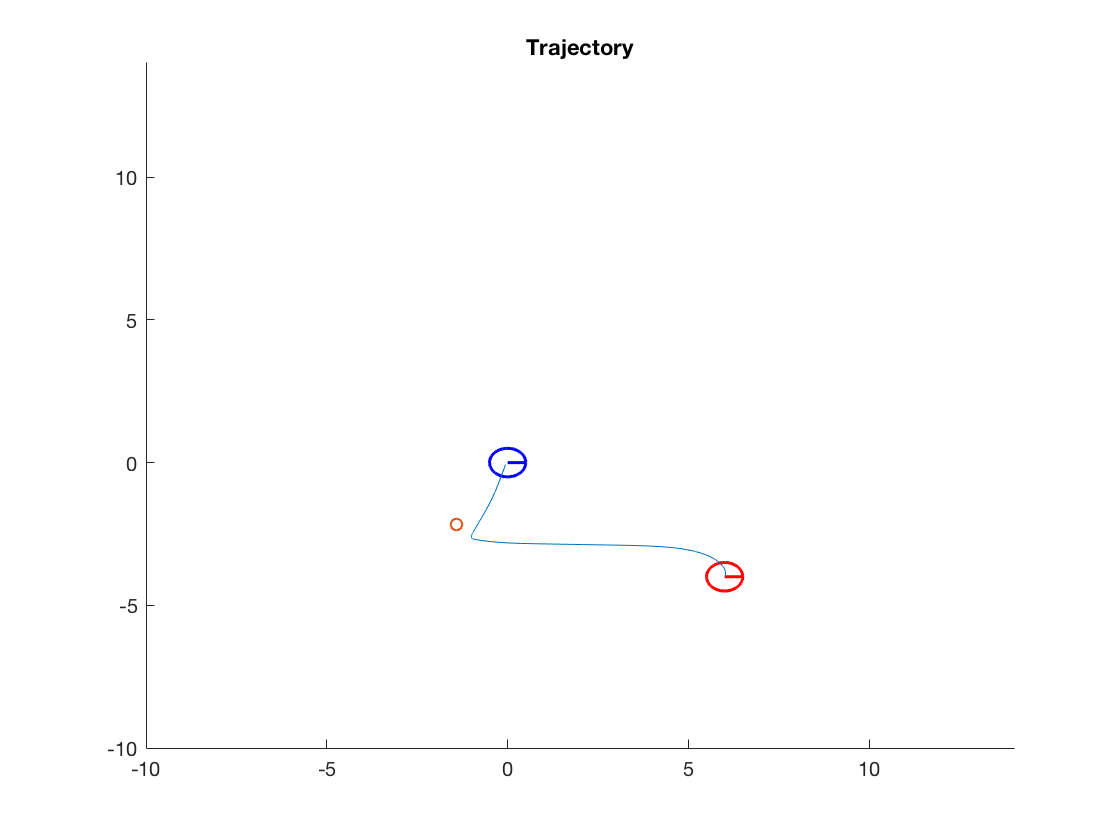
\includegraphics[scale=0.15]{possible_trajectory.png} 
%\caption{Trajectory of the robot  \label{fig:r}} 
%\end{subfigure}
%\begin{subfigure}[t]{0.32\textwidth}
%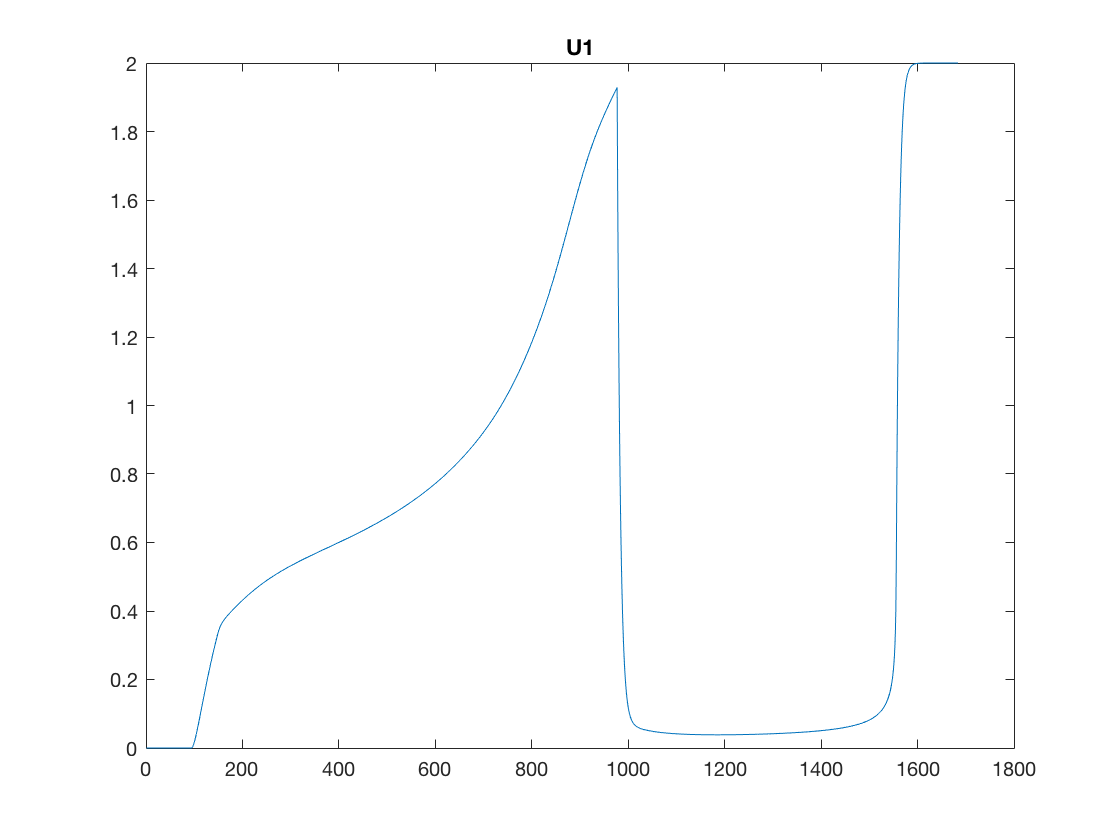
\includegraphics[scale=0.15]{U1.png} 
%\caption{The linear velocity of the robot \label{fig:theta}} 
%\end{subfigure}
%\begin{subfigure}[t]{0.32\textwidth}
%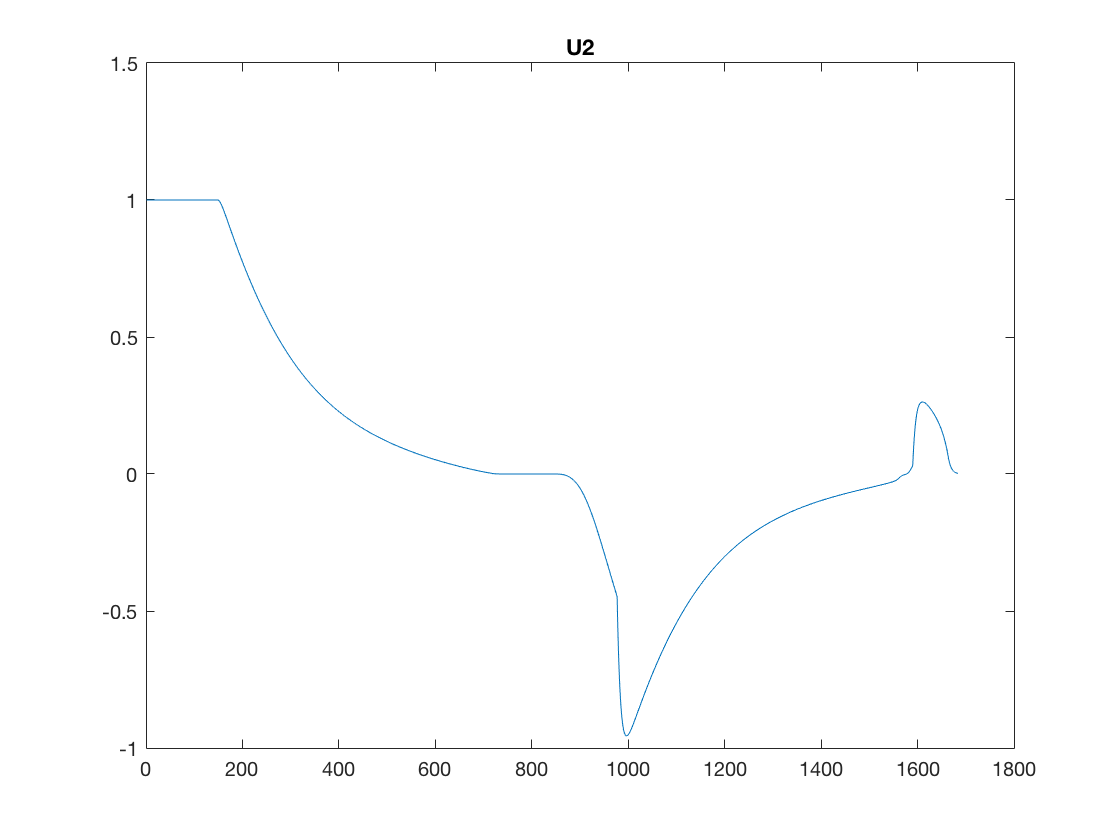
\includegraphics[scale=0.15]{U2.png} 
%\caption{The angular velocity of the robot \label{fig:delta}} 
%\end{subfigure}
%\caption{The above figures show the trajectory, linear velocity and angular velocity of the robot while avoiding the obstacle.\label{fig:state}}
%\end{figure*}
The last two elements in the diagonal of $H$ were chosen to be zero to ensure that the negative quadratic cost of the slack variables $\alpha_1$ and $\alpha_2$ is as large as possible. Conversely, the last two elements of $F^T$ were chosen to ensure that $\alpha_1$ and $\alpha_2$ were negative to minimize the cost.

The control Lyapunov functions $V_1$ and $V_2$ are the Lyapunov functions corresponding to the objectives of driving the state to zero and enforcing the steering control respectively; the equations are given by 
\begin{equation}
V_1=\frac{1}{2}(r^2+\theta^2)
\end{equation} and
\begin{equation}
V_2=\frac{1}{2}z_*^2.
\end{equation}
$z_*$ in $V_2$ represents the different steering objectives $z_1$ and $z_2$ in \eqref{z1} and \eqref{z2}. Because there are two steering objectives, two QP control laws are required: one which drives the state towards the target while avoiding obstacles, and the other that drives the state in such a way that the robot steers away from obstacles. Toggling between steering objectives is dependent on the obstacle measurement. If the measurement of the distance between the robot and the obstacle was less than the minimum safe distance, then the steering objective $z_2$ is used. Otherwise, $z_1$ is used, and $\alpha_1=0$ is additionally enforced. $h(x)$ and $B$ in the QP controller are given in equations \eqref{zbf} and \eqref{bf}. 

\section{Results}
MATLAB simulation was used to verify that the navigation control strategy using the QP controller enabled the robot to navigate to the desired position while avoiding obstacles. Figure~\ref{fig:octoplot} shows that the navigation control strategy is capable of driving the robot to the final position while avoiding obstacles from a variety of starting locations. Figure~\ref{fig:prm_works} shows that the navigation control strategy enables safe navigation between target waypoints generated through a probabilistic roadmap.

Implementing the navigation control law in the ROS framework, Gazebo simulation, shown in Figure~\ref{fig:gazebo}, was used to corroborate the results of the MATLAB simulation. Following success in Gazebo, robot experiments were performed on the Segway robot ``Jeeves''. The Hokuyo laser scans are subscribed to and the appropriate processing is performed. The robot is commanded to drive to a set point and the optimal $u$ is computed at every time step. The dynamics is propogated forward using the odometry. To add the obstacle, a human moved into the operation range of the obstacle as can be seen in Figure \ref{fig:jeeves_exp} and ensured that the robot did not break any safety constraints. A video showing one experimental run can be seen at \url {https://youtu.be/uhTiYyZxtfc}. The video shows that the robot maintains its safe distance from the human and tries to avoid the human, when the human walks out of the radius of influence the robot is free to move at greater speeds again.

\begin{figure}[h!]
\centering
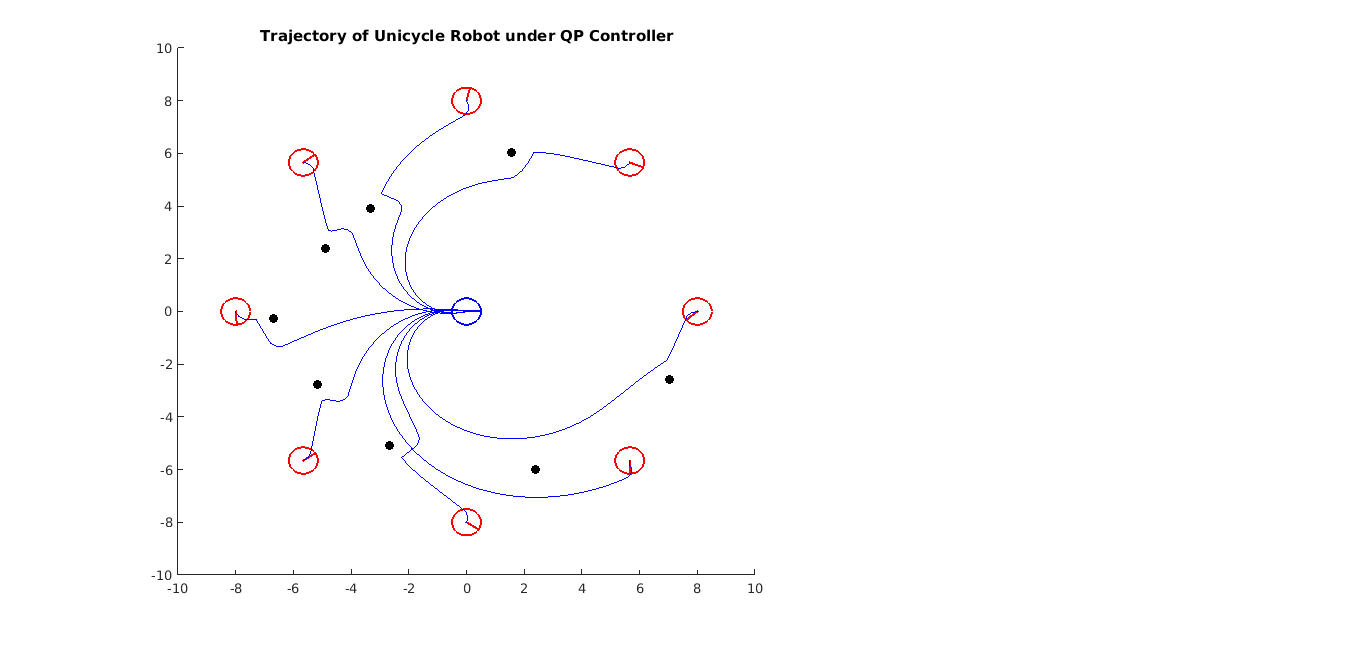
\includegraphics[scale=0.3]{octoPlotProofEditSqur.png} 
\caption{The figure above shows the same initializations at eight different starting locations and the trajectories followed by the robot to the origin to show that the robot can generate a trajectory from an arbitrary initial condition to the origin while avoiding the obstacle.\label{fig:octoplot}} 
\end{figure}

\begin{figure}[h!]
\centering
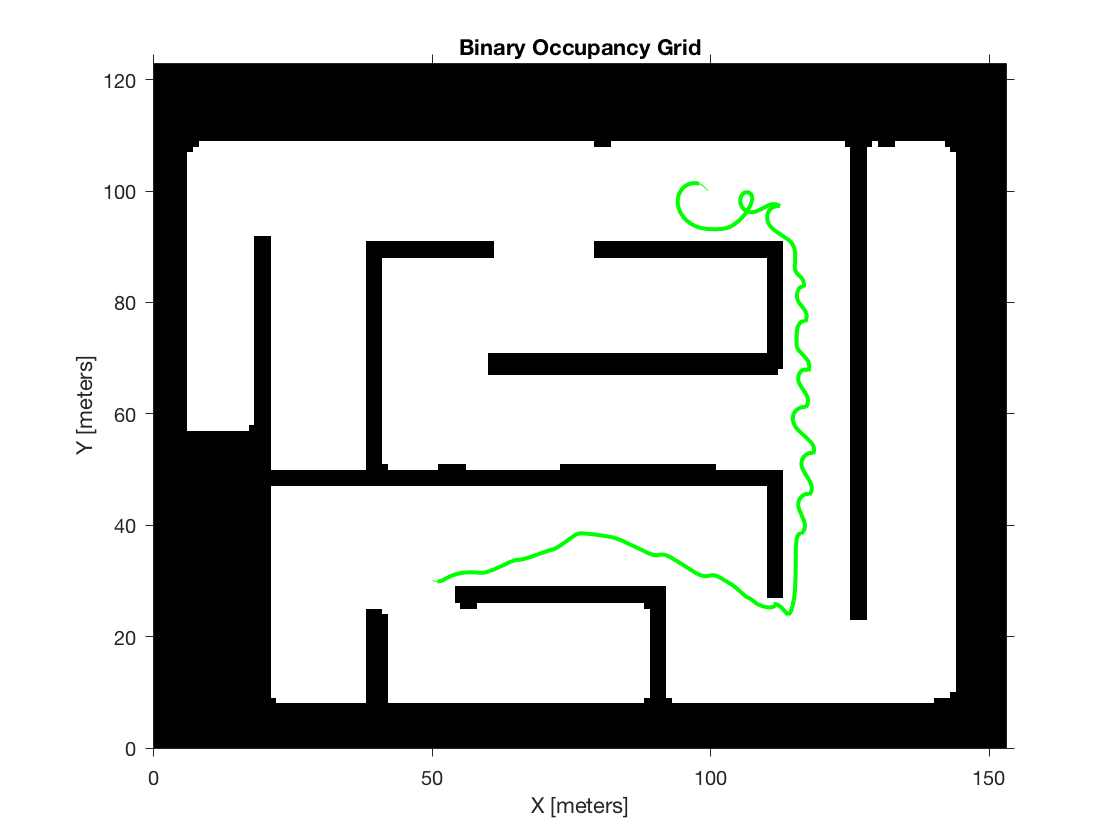
\includegraphics[scale=0.18]{thick_plot.png} 
\caption{Safe Navigation under QP Controller with Barrier Functions\label{fig:prm_works}}
\end{figure}

\begin{figure}[h!]
\centering
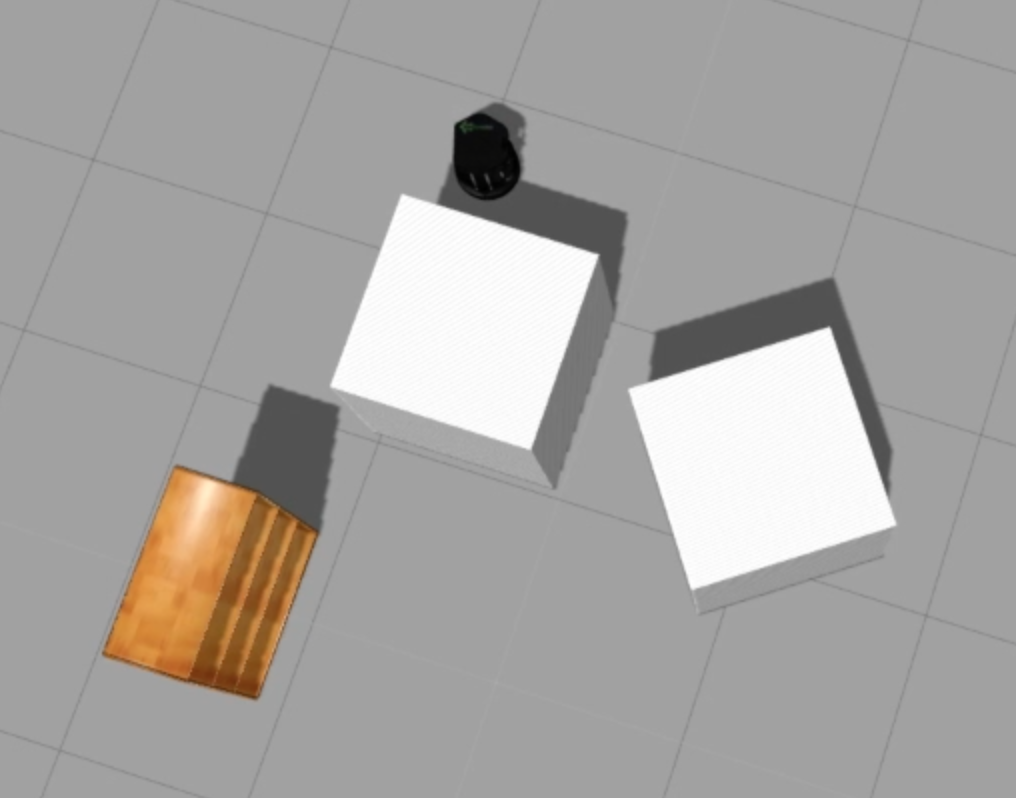
\includegraphics[scale=0.3]{Gazebo_exp.png} 
\caption{Gazebo Simulation Navigation\label{fig:gazebo}}
\end{figure}

\begin{figure}[h!]
\centering
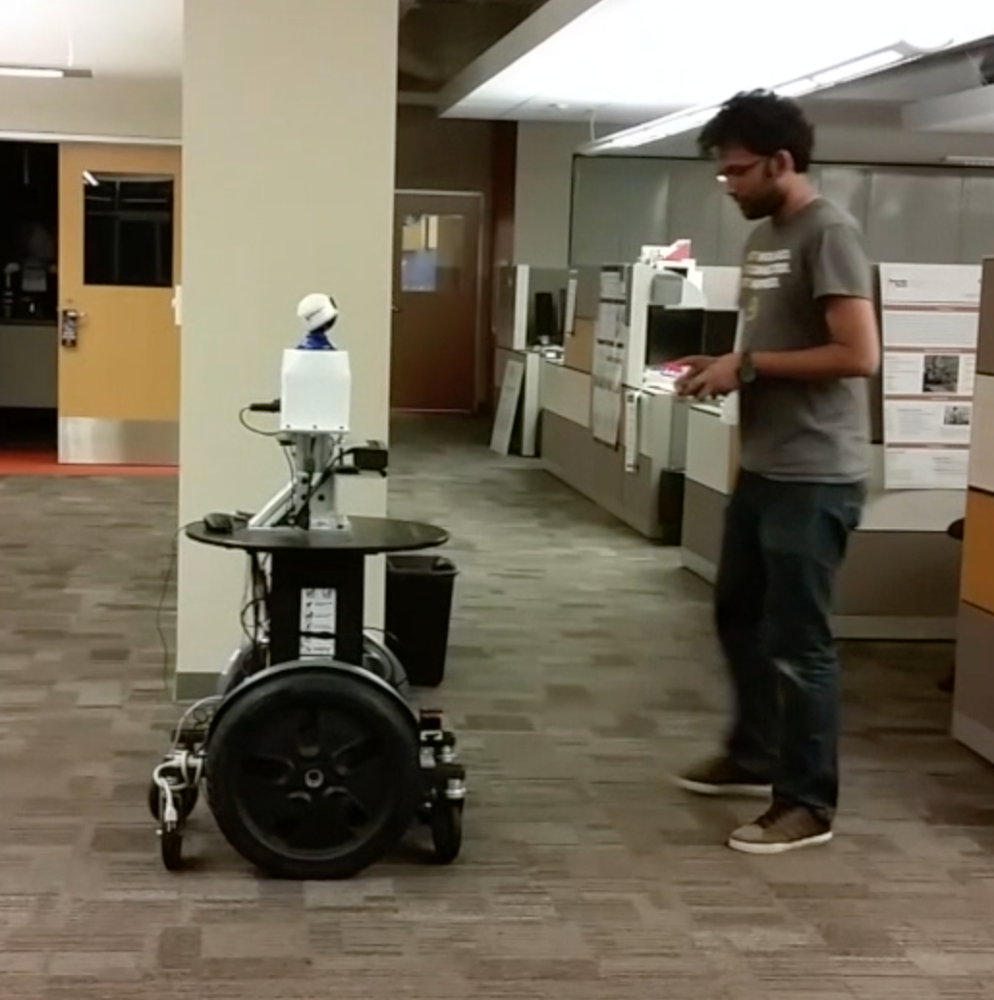
\includegraphics[scale=0.13]{jeeves_exp.png} 
\caption{Real robot experiment with the segway RMP robot. The robot is stopped at a safe distance from the human obstacle. \label{fig:jeeves_exp}}
\end{figure}


\section{Conclusion}
We show that the nonlinear controller is generatlizable to multiple robots and is provably safe. The theoretical analysis shows that the controller stabilizes the system while obeying the ``safety'' rules. The exaperimental analysis shows that the system can be implemented on a real world system and the results are consistent with the claims. The developed system is almost self-contained and does not require many parameter adjustments. 
For future work, we propose more complex modelling of the obstacles to better capture the nature of the obstacle. For example, the safety barrier around a human is different from that around a wall. It is more ``socially'' acceptable to drive close to a wall but not as acceptable to be that close to a human.

\bibliographystyle{plainnat}
\bibliography {bibi}



%% Use plainnat to work nicely with natbib. 




\end{document}


